%%% Lecture 1 Slides %%%

\documentclass{beamer}

%\documentclass[handout]{beamer}
%\usepackage{pgfpages}
%\pgfpagesuselayout{2 on 1}[a4paper,border shrink=5mm]
%\pgfpagesuselayout{1 on 1}[a4paper,border shrink=5mm]



\usepackage{amssymb}
\usepackage{amsmath}


\newcommand{\bs}{\boldsymbol}
\newcommand{\mb}{\mathbf}
\newcommand{\indep}{{\bot\negthickspace\negthickspace\bot}}
\newcommand{\notindep}{{\bot\negthickspace\negthickspace\bot}{\negthinspace
  \negmedspace \negthickspace \negthickspace \diagup
  \;}}
\renewcommand{\S}{\mb{S}}

%\usepackage{pdfpages}
%\pdfpagelayout{2 on 1}

\mode<presentation>
{
  \usetheme{Singapore}    %Warsaw}
  % or ...

  \setbeamercovered{transparent}
  % or whatever (possibly just delete it)
}


\usepackage[english]{babel}
% or whatever

\usepackage[latin1]{inputenc}
% or whatever

\usepackage{times}
\usepackage[T1]{fontenc}
% Or whatever. Note that the encoding and the font should match. If T1
% does not look nice, try deleting the line with the fontenc.


\title[QTM 220] % (optional, use only with long paper titles)
{QTM 220}

\subtitle
{Conditionally Randomized Experiments and Natural Experiments} 

\date{December 4 and 6, 2018}%[Short Occasion] % (optional)


\subject{Talks}
% This is only inserted into the PDF information catalog. Can be left
% out. 



% If you have a file called "university-logo-filename.xxx", where xxx
% is a graphic format that can be processed by latex or pdflatex,
% resp., then you can add a logo as follows:

% \pgfdeclareimage[height=0.5cm]{university-logo}{university-logo-filename}
% \logo{\pgfuseimage{university-logo}}



% Delete this, if you do not want the table of contents to pop up at
% the beginning of each subsection:

\AtBeginSection[]
{
  \begin{frame}<beamer>
    \frametitle{Outline}
    \tableofcontents[currentsection,currentsubsection]
  \end{frame}
}


\AtBeginSubsection[]
{
  \begin{frame}<beamer>
    \frametitle{Outline}
    \tableofcontents[currentsection,currentsubsection]
  \end{frame}
}


% If you wish to uncover everything in a step-wise fashion, uncomment
% the following command: 

%\beamerdefaultoverlayspecification{<+->}


\begin{document}

\begin{frame}
  \titlepage
\end{frame}

\begin{frame}
  \frametitle{Outline}
  \tableofcontents
  % You might wish to add the option [pausesections]
\end{frame}

\section{Conditionally/Blocked Randomized Experiments}


\frame{
\frametitle{(Marginally) Randomized Experiments}

\begin{itemize}
\item<1-> Units/individuals are randomly assigned to treatment or control.
\item<2-> Work great with large sample sizes and often work fine with medium sample sizes.  
\item<3-> With small/medium sample sizes, can get unlucky randomizations. 
\item<4-> In the blood pressure example, if we get unlucky we might assign treatment to young subjects and control to older subjects, hence treatment confounded by age.
\item<5-> Can try to fix unlucky randomizations by controlling for age, but if treatment and age close to collinear, then VIF large.
\end{itemize}

}

\frame{
\frametitle{Conditionally/Blocked Randomized Experiments}

\begin{itemize}
\item<1-> Units/individuals are randomly assigned to treatment or control within blocks (e.g., randomly assign among young, and randomly assign among old).  
\item<2-> Ensures some young and old assigned to both treatment and control.
\item<4-> Can use different probability of treatment assignment in the block (e.g. 50-50 among young and 75-25 among old)
\item<5-> Observational studies can sometimes be thought of as approximations of conditionally randomized experiments.
\end{itemize}

}

\frame{
\frametitle{Control Variables}

In a marginally randomized experiment,
\begin{itemize}
\item Simple regression of $Y$ on $T$ will be unbiased.
\item Multiple regression of $Y$ on $T$ and $X$ can be more efficient (especially in large samples).
\item Bias/Variance tradeoff.
\end{itemize}


In a conditionally randomized experiment,
\begin{itemize}
\item Simple regression of $Y$ on $T$ will be biased when probability of treatment assignment differs across blocks.
\item Multiple regression of $Y$ on $T$ and $X$ almost always more efficient.
\end{itemize}

}


\frame{
\frametitle{Example: Conditionally Randomized Experiments}


If treatments are randomly assigned conditionally on another variable, then the average $Y_i(1)$ among the $T_i=1$ subjects \alert{may not} equal the average $Y_i(1)$ among the $T_i=0$ subjects.

\begin{center}
\begin{tabular}{ccc|ccc}
$i$ & $T_i$ & $Y_i$ & $Y_i(1)$ & $Y_i(0)$ & $Y_i(1)-Y_i(0)$ \\
\hline
1 & 1 & 70 & 70 & \alert{70} & \alert{0} \\
2 & 1 & 80 & 80 & \alert{70} & \alert{10} \\
3 & 0 & 60 & \alert{{\bf 60}} & 60 & \alert{{\bf0}} \\
4 & 0 & 70 & \alert{80} & 70 & \alert{10} \\
5 & 0 & 70 & \alert{70} & 70 & \alert{0} \\
6 & 0 & 80 & \alert{80} & 80 & \alert{0} \\
\end{tabular}
\end{center}


\visible<1-2>{What is the average $Y_i(1) - Y_i(0)$?} 
\visible<2>{
\begin{align*}
\frac{\alert{0} + \alert{10} + \alert{0} +  \alert{10} +\alert{0} +\alert{0}}{6}  &= \frac{20}{6}\\
&\approx 3.3\\
 &\ne 75 - 70
\end{align*}}


}



\frame{
\frametitle{Example: Conditionally Randomized Experiment}


Suppose for one group ($\textcolor{green}{X=1}$) a coin was flipped to assign treatment to half of the units, and for another group ($\textcolor{blue}{X=0}$), one out of four units was assigned to treatment.   

\begin{center}
\begin{tabular}{cccc|ccc}
$i$ & $X_i$ & $T_i$ & $Y_i$ & $Y_i(1)$ & $Y_i(0)$ & $Y_i(1)-Y_i(0)$ \\
\hline
1 & \textcolor{blue}{0} &1 & 70 & \textcolor{blue}{70} & ? & ? \\
2 & \textcolor{green}{1} &1 & 80 & \textcolor{green}{80} & ? & ? \\
3 & \textcolor{blue}{0} & 0 & 60 & ? & \textcolor{blue}{60} &?\\
4 & \textcolor{green}{1} &0& 70 & ? & \textcolor{green}{70} & ? \\
5 & \textcolor{blue}{0} & 0&70 & ? & \textcolor{blue}{70} & ? \\
6 & \textcolor{blue}{0}& 0 & 80 & ? & \textcolor{blue}{80} & ? \\
\end{tabular}
\end{center}

}

\frame{
\frametitle{Example: Conditionally Randomized Experiment}


Suppose for one group ($\textcolor{green}{X=1}$) a coin was flipped to assign treatment to half of the units, and for another group ($\textcolor{blue}{X=0}$), one out of four units was assigned to treatment.   

\begin{center}
\begin{tabular}{cccc|ccc}
$i$ & $X_i$ & $T_i$ & $Y_i$ & $Y_i(1)$ & $Y_i(0)$ & $Y_i(1)-Y_i(0)$ \\
\hline
1 & \textcolor{blue}{0} &1 & 70 & \textcolor{blue}{70} & \alert{70} & \alert{0} \\
2 & \textcolor{green}{1} &1 & 80 & \textcolor{green}{80} & \alert{70} & \alert{10} \\
3 & \textcolor{blue}{0} & 0 & 60 & \alert{60} & \textcolor{blue}{60} & \alert{0}\\
4 & \textcolor{green}{1} &0& 70 & \alert{80} & \textcolor{green}{70} & \alert{10} \\
5 & \textcolor{blue}{0} & 0&70 & \alert{70} & \textcolor{blue}{70} & \alert{0} \\
6 & \textcolor{blue}{0}& 0 & 80 & \alert{80} & \textcolor{blue}{80} & \alert{0} \\
\end{tabular}
\end{center}


\visible<1-2>{What is the average $Y_i(1)$ among the $X=0$ subjects?} 
\visible<2>{$$
\frac{\textcolor{blue}{70} +\alert{60} +\alert{70} + \alert{80}}{4}  = 70
$$}
\vspace{-2.4cm}

\visible<3-4>{What is the average $Y_i(1)$ among the $X=0$, $T=1$ subjects?} 
\visible<4>{$$
\frac{\textcolor{blue}{70} }{1}  = 70
$$}
\vspace{-2.4cm}

\visible<5-6>{What is the average $Y_i(1)$ among the $X=1$ subjects?} 
\visible<6>{$$
\frac{\textcolor{green}{80} +\alert{80} }{2}  = 80
$$}
\vspace{-2.4cm}

\visible<7-8>{What is the average $Y_i(1)$ among the $X=1$, $T=1$ subjects?} 
\visible<8>{$$
\frac{\textcolor{green}{80}}{1}  = 80
$$}

}






\frame{
\frametitle{Example: Conditionally Randomized Experiment }


If we analyze each experiment separately, and average the results by the proportion in each experiment, then we get the ATE.

\begin{center}
\begin{tabular}{cccc|ccc}
$i$ & $X_i$ & $T_i$ & $Y_i$ & $Y_i(1)$ & $Y_i(0)$ & $Y_i(1)-Y_i(0)$ \\
\hline
1 & \textcolor{blue}{0} &1 & 70 & \textcolor{blue}{70} & ? & ? \\
2 & \textcolor{green}{1} &1 & 80 & \textcolor{green}{80} & ? & ? \\
3 & \textcolor{blue}{0} & 0 & 60 & ? & \textcolor{blue}{60} &?\\
4 & \textcolor{green}{1} &0& 70 & ? & \textcolor{green}{70} & ? \\
5 & \textcolor{blue}{0} & 0&70 & ? & \textcolor{blue}{70} & ? \\
6 & \textcolor{blue}{0}& 0 & 80 & ? & \textcolor{blue}{80} & ? \\
\end{tabular}
\end{center}



\begin{align*}
\textcolor{blue}{\frac{4}{6}} \cdot \left\{\frac{70}{1} -  \frac{60+70+80}{3}\right\} &+ \textcolor{green}{\frac{2}{6}} \cdot \left\{\frac{80}{1} -  \frac{70}{1}\right\} \\
&= \frac{20}{6}
\end{align*}
}


\frame{
\frametitle{Example: Conditionally Randomized Experiment }


If we analyze each experiment separately, and average the results by the proportion in each experiment, then we get the ATE.


\begin{center}
\begin{tabular}{cccc|ccc}
$i$ & $X_i$ & $T_i$ & $Y_i$ & $Y_i(1)$ & $Y_i(0)$ & $Y_i(1)-Y_i(0)$ \\
\hline
1 & \textcolor{blue}{0} &1 & 70 & \textcolor{blue}{70} & \alert{70} & \alert{0} \\
2 & \textcolor{green}{1} &1 & 80 & \textcolor{green}{80} & \alert{70} & \alert{10} \\
3 & \textcolor{blue}{0} & 0 & 60 & \alert{60} & \textcolor{blue}{60} & \alert{0}\\
4 & \textcolor{green}{1} &0& 70 & \alert{80} & \textcolor{green}{70} & \alert{10} \\
5 & \textcolor{blue}{0} & 0&70 & \alert{70} & \textcolor{blue}{70} & \alert{0} \\
6 & \textcolor{blue}{0}& 0 & 80 & \alert{80} & \textcolor{blue}{80} & \alert{0} \\
\end{tabular}
\end{center}



\begin{align*}
\textcolor{blue}{\frac{4}{6}} \cdot \left\{\frac{70}{1} -  \frac{60+70+80}{3}\right\} &+ \textcolor{green}{\frac{2}{6}} \cdot \left\{\frac{80}{1} -  \frac{70}{1}\right\} \\
&= \frac{20}{6} = \frac{\alert{10}+\alert{10}}{6}
\end{align*}
}



\frame{
\frametitle{Conditional Exchangeability}


With a conditionally randomized experiment, the conditional exchangeability/unconfoundedness assumption allows us to relate average potential outcomes to average observed outcomes.


\visible<2->{\begin{align*}
E[Y_i(1)|X_i=x] &= E[Y_i(1)|T_i=1,X_i=x] \\
 &= E[Y_i|T_i=1,X_i=x]  \\
\end{align*}}

%\vspace{-2.8cm}

\visible<3->{\begin{align*}
E[Y_i(0)|X_i=x] &= E[Y_i(0)|T_i=0,X_i=X] \\
 &= E[Y_i|T_i=0,X_i=X]  \\
\end{align*}}
\visible<4>{Note this was also true for a (marginally) randomized experiment.}

}

\frame{
\frametitle{(Marginal) Exchangeability}


With a conditionally randomized experiment, the (marginal) exchangeability/unconfoundedness assumption does not hold in general.

\visible<2->{\begin{align*}
E[Y_i(1)] &\ne E[Y_i(1)|T_i=1] \\
 &= E[Y_i|T_i=1]  \\
\end{align*}}

%\vspace{-2.8cm}

\visible<3->{\begin{align*}
E[Y_i(0)] &\ne E[Y_i(0)|T_i=0] \\
 &= E[Y_i|T_i=0]  \\
\end{align*}}
\visible<4->{Note that these would hold for a (marginally) randomized experiment.}


}




\frame{
\frametitle{Estimation with Conditionally Randomized Experiments (Binary X)}

With a binary $T$ and a binary $X$, we can always write the conditional expectation as a linear interactive function,

\begin{align*}
E[Y|T=t,X=x] &= \beta_0 + \beta_1 \cdot t + \beta_2 \cdot x + \beta_3 \cdot t \cdot x \\
\visible<2->{E[Y|T=0,X=0] &= \beta_0} \\
\visible<3->{E[Y|T=1,X=0] &= \beta_0 + \beta_1} \\
\visible<4->{E[Y|T=0,X=1] &= \beta_0 + \beta_2} \\
\visible<5->{E[Y|T=1,X=1] &= \beta_0 + \beta_1 + \beta_2 + \beta_3}
\end{align*}


}

\frame{
\frametitle{Interpretation with Conditionally Randomized Experiments (Binary X)}

Therefore, when $T$ is randomized conditionally on $X$,
\begin{align*}
E[Y|T=1,X=0]-E[Y|T=0,X=0] &= (\beta_0 + \beta_1) - \beta_0 \\
&= \beta_1
\end{align*}
can be interpreted as the CATE among the $X=0$ subjects. \pause
\begin{align*}
E[Y|T=1,X=1]&-E[Y|T=0,X=1] = \\
&(\beta_0 + \beta_1 + \beta_2 + \beta_3) - (\beta_0 + \beta_2) \\
&= \beta_1+\beta_3
\end{align*}
can be interpreted as the CATE among the $X=1$ subjects. \pause
\begin{align*}
E[ \beta_1+\beta_3 \cdot X] &= \beta_1+\beta_3 \cdot E[X]\\
&= (1-E[X]) \beta_1 +  E[X] (\beta_1+\beta_3)
\end{align*}
can be interpreted as the ATE


}

\frame{
\frametitle{Interpretation with Conditionally Randomized Experiments (Non-binary X)}

When $T$ is randomized conditionally on $X$, under a linear model 
\begin{align*}
E[Y|T=t,X=x] &= \beta_0 + \beta_1 \cdot t + \beta_2 \cdot x + \beta_3 \cdot t \cdot x \\
&= \beta_0 + \beta_2 \cdot x + (\beta_1  + \beta_3 \cdot x) \cdot t 
\end{align*}
and the slope in the $t$ direction can be interpreted as the CATE among the $X=x$ subjects.
\begin{align*}
E[Y|T=1,X=x]-E[Y|T=0,X=x] &= (\beta_1  + \beta_3 \cdot x)
\end{align*}
 \pause


By averaging these CATES over the values of $X$, we get the ATE
\begin{align*}
E[\beta_1 + \beta_3 \cdot X] &= \beta_1+\beta_3 \cdot E[X]\\
\end{align*}

}





\frame{
\frametitle{Inference with Conditionally Randomized Experiments}

If $\beta_3=0$, and the four descriptive assumptions hold, then we can get approximate CIs and tests for the ATE by running the additive regression of $Y$ on $T$ and $X$.\\ \pause

\vspace{.8cm}

If $\beta_3 \ne 0$, and the four descriptive assumptions hold  then we can get approximate CIs and tests for the ATE by subtracting the mean $E[X]$ off of all $X$ values, running the interactive regression of $Y$ on $T$, $X-E[X]$, and $T\cdot (X-E[X])$ and using the estimate and standard error associated with coefficient on $T$. \pause

\vspace{.8cm}

If $\beta_3 \ne 0$, and the four descriptive assumptions hold  then can get approximate CIs and tests for a weighted ATE by running the additive regression of $Y$ on $T$ and $X$.



}


%\begin{subsection}{Modern and Classical Assumptions}


%\frame{
%\frametitle{Unconfoundedness in a Conditionally Randomized Experiment}
%
%
%With randomization conditional on $X$, the unconfoundedness/error term assumption will hold conditional on $X$. 
%
%\begin{align*}
%Y_i &= T_i Y_i(1) + (1-T_i) Y_i(0)\\
%&= Y_i(0) +  (Y_i(1)-Y_i(0)) T_i\\
%&= \beta_{0i} + \beta_{1i} T_i \\
%&= \beta_{0} + \beta_{1i} T_i + \epsilon_i
%\end{align*}
%
%\visible<2>{\begin{align*}
%E[Y_i(1)|X=x] &= E[Y_i(1)|T=1,X=x] \\
% \beta_{0} + \beta_{1} + E[\epsilon_i|X=x] &= \beta_{0} + \beta_{1} + E[\epsilon_i|T=1|X=x] \\
%\end{align*}}
%
%\vspace{-2.8cm}
%
%\visible<3>{\begin{align*}
%E[Y_i(0)|X=x] &= E[Y_i(0)|T=1,X=x] \\
% \beta_{0} + E[\epsilon_i|X=x] &= \beta_{0} + E[\epsilon_i|T=1,X=x] \\
%\end{align*}}
%
%}






%\frame{
%\frametitle{Interpreting the Multiple Regression Model}
%
%Consider the multiple regression model from ALZ page 158.
%\visible<1>{\begin{align*}
%Y_i &= \beta_{0} + \beta_{1} X_{1i} + \beta_{2} X_{2i} + \dots +  \beta_{k} X_{ki}  + \epsilon_i
%\end{align*}}
%
%\vspace{-2cm}
%
%\visible<2->{\begin{align*}
%Y_i &= \beta_{0} + \beta_{1} X_{1i} + \beta_{2} X_{2i} + \epsilon_i
%\end{align*}}
%
%\begin{itemize}
%\item<3->  Should we interpret both $\beta_{1}$ and $\beta_{2}$ as causal effects?
%\item<4->  If so, would this interpretation be justified if $X_{1}$ were randomized conditionally on $X_{2}$?
%\item<5->  What randomized experiment would justify this interpretation?
%\end{itemize}
%
%
%}



\section{Example of a ``Natural'' Experiment}


\frame{
\frametitle{Washington (2008) example}

Washington (2008) examines the effect of having daughters on the AAUW scores for members of congress (MCs) by comparing MCs with more daughters to MCs with fewer daughters, conditional on family size.


}

\frame{
\frametitle{Omitted Variable Bias}

Suppose we believe that a two variable linear model is the true model in the Washington (2008) example,
\begin{align*}
Y_i &= \beta_0 + \beta_1 Girls_i + \beta_2 Children_i + \epsilon_i
\end{align*}
but suppose that we omit the $Children$ variable from the analysis
 \begin{align*}
Y_i &= \beta_0^{*} + \beta_1^{*} Girls_i + \epsilon_i^{*}
\end{align*}

}


\frame{

If we write the model for children as the following: 
\begin{align*}
Children_i &= \gamma_0 + \gamma_1 Girls_i + \nu_i
\end{align*}
then the two explanatory variable model can be re-written as the following:


\begin{align*}
Y_i &= \beta_0 + \beta_1 Girls_i + \beta_2 Children_i + \epsilon_i \\
&= \beta_0 + \beta_1 Girls_i + \beta_2 (\gamma_0 + \gamma_1 Girls_i + \nu_i) + \epsilon_i \\
&= \underbrace{\beta_0 + \beta_2 \gamma_0}_{\beta_0^{*}} + \underbrace{(\beta_1 + \beta_2 \gamma_1)}_{\beta_1^{*}} Girls_i + \underbrace{\epsilon_i + \beta_2 \nu_i}_{\epsilon_i^{*}}
\end{align*}
%this implies that $\beta_1^{*} = (\beta_1 + \beta_2 \gamma_1)$ and $\beta_2 \gamma_1$ describes the bias due to omitting the $Children$ variable from the model. Using the 105th congress and the AAUW scores, we can see the results of this bias. In the multiple regression model, the effect of an extra girl (conditional on number of children) is estimated to increase AAUW score by almost 6 points ($\widehat{\beta}_1= 5.776$). However, if we fail to condition on the number of children, the effect of an extra girl is estimated to decrease AAUW score by almost 3 points ($\widehat{\beta}_1^{*}= -2.784$).

}

\frame{
\frametitle{Other Conditional Models}

What are some other ways to model the Washington (2008) example?
\begin{align*}
Y_i &= \beta_0 + \beta_1 Girls_i + \beta_2 Children_i + \epsilon_i
\end{align*} \pause

\vspace{.5cm}

Equation 1 from Washington (2008) re-written:
\begin{align*}
Y_i = \beta_0 + \beta_1 Girls_i &+ \beta_2 1_{\{Children_i =1\}} \\
&+ \beta_3 1_{\{Children_i =2\}} \\
&+ \vdots \\
&+ \beta_6 1_{\{Children_i =5\}} + \epsilon_i
\end{align*}



}

\frame{
\frametitle{The Additive Linear Model (105th Congress)}

\begin{figure}[ht]
  \begin{center}
    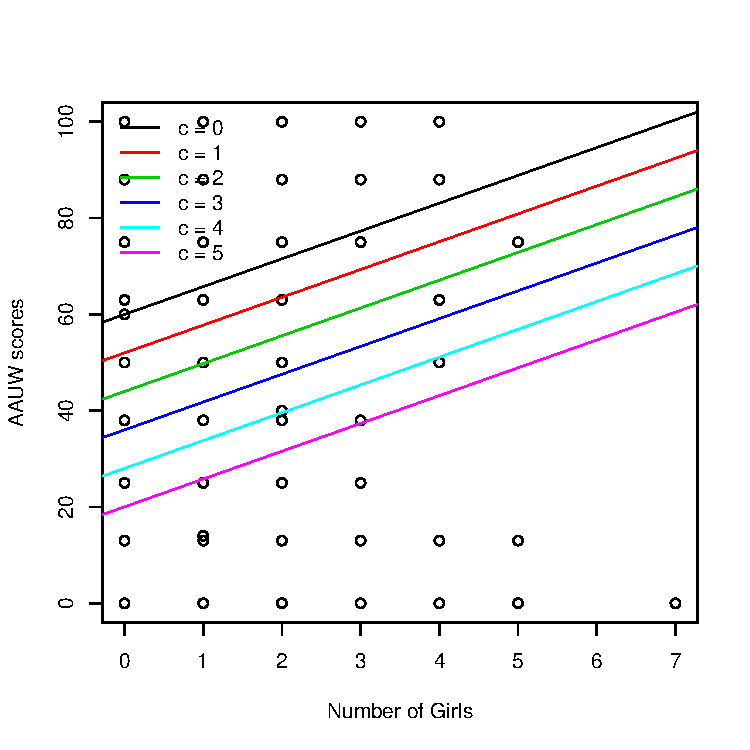
\includegraphics[height=2.5in]{3e.pdf}
  \end{center}
  \vspace{-0.275in}
\end{figure}  \pause

How would this picture change if we used the model in Equation 1 of Washington (2008)?

}

 \frame{
\frametitle{Washington (2008) Eq. 1 Model}

\begin{figure}[ht]
  \begin{center}
    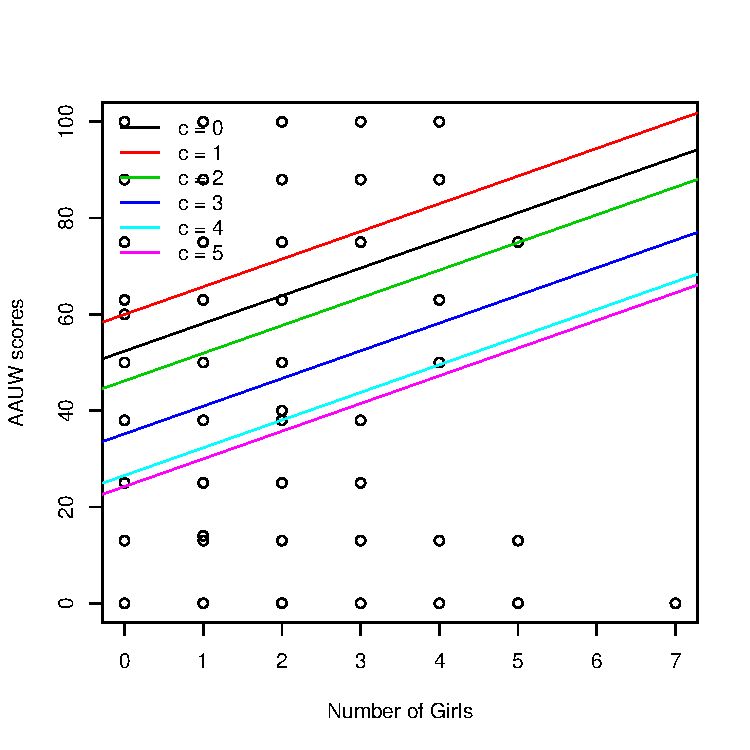
\includegraphics[height=2.5in]{WashingtonEq1.pdf}
  \end{center}
  \vspace{-0.275in}
\end{figure} 

}


%\frame{
%\frametitle{Points of Potential Confusion}
%
%Is $\beta_1^{*}$ meant to be causal? \\
% \begin{align*}
%Y_i &= \beta_0^{*} + \beta_1^{*} Girls_i + \epsilon_i^{*}
%\end{align*}
%
%\pause
%
%\vspace{.5cm}
%
%Is $\gamma_1$ meant to be causal?
%\begin{align*}
%Children_i &= \gamma_0 + \gamma_1 Girls_i + \nu_i
%\end{align*}
%
%\pause
%
%\vspace{.5cm}
%
%If $\gamma_1$ were meant to be causal would we want to include the omitted variable?
%
%}
%
%
%\frame{
%\frametitle{Some Typical Econometric Advice}
%
%
%
%\begin{quote}
%In sum, if the variable we leave out is positively correlated with the variable we include and also has itself a positive effect on the dependent variable, then our mispecified model will produce an upward-biased estimator of the effect of $X_1$ on $Y$. [Ashenfelter, Levine, and Zimmerman, p. 189]%\cite[p. 449]{Kme86}
%\end{quote}
%
%\pause
%
%
%
%\begin{quote}
%The short answer to the questions posed above is that the OLS estimates based on the equation containing too many explanatory variables will indeed be unbiased estimates of the true parameters. [Ashenfelter, Levine, and Zimmerman, p. 187]%\cite[p. 449]{Kme86}
%\end{quote}
%
%
%%\begin{quote}
%%The conclusion, then, is that if the specification error consists of
%%including some irrelevant explanatory variables in the regression
%%equation, the least squares estimators of the regression coefficients
%%are unbiased but not efficient.  [Kmetka 1986, p. 449]%\cite[p. 449]{Kme86}
%%\end{quote}
%
%
%}
%
%
%
%\frame{
%\frametitle{Directed Acyclic Graphs}
%
%\begin{figure}[ht]
%  \begin{center}
%    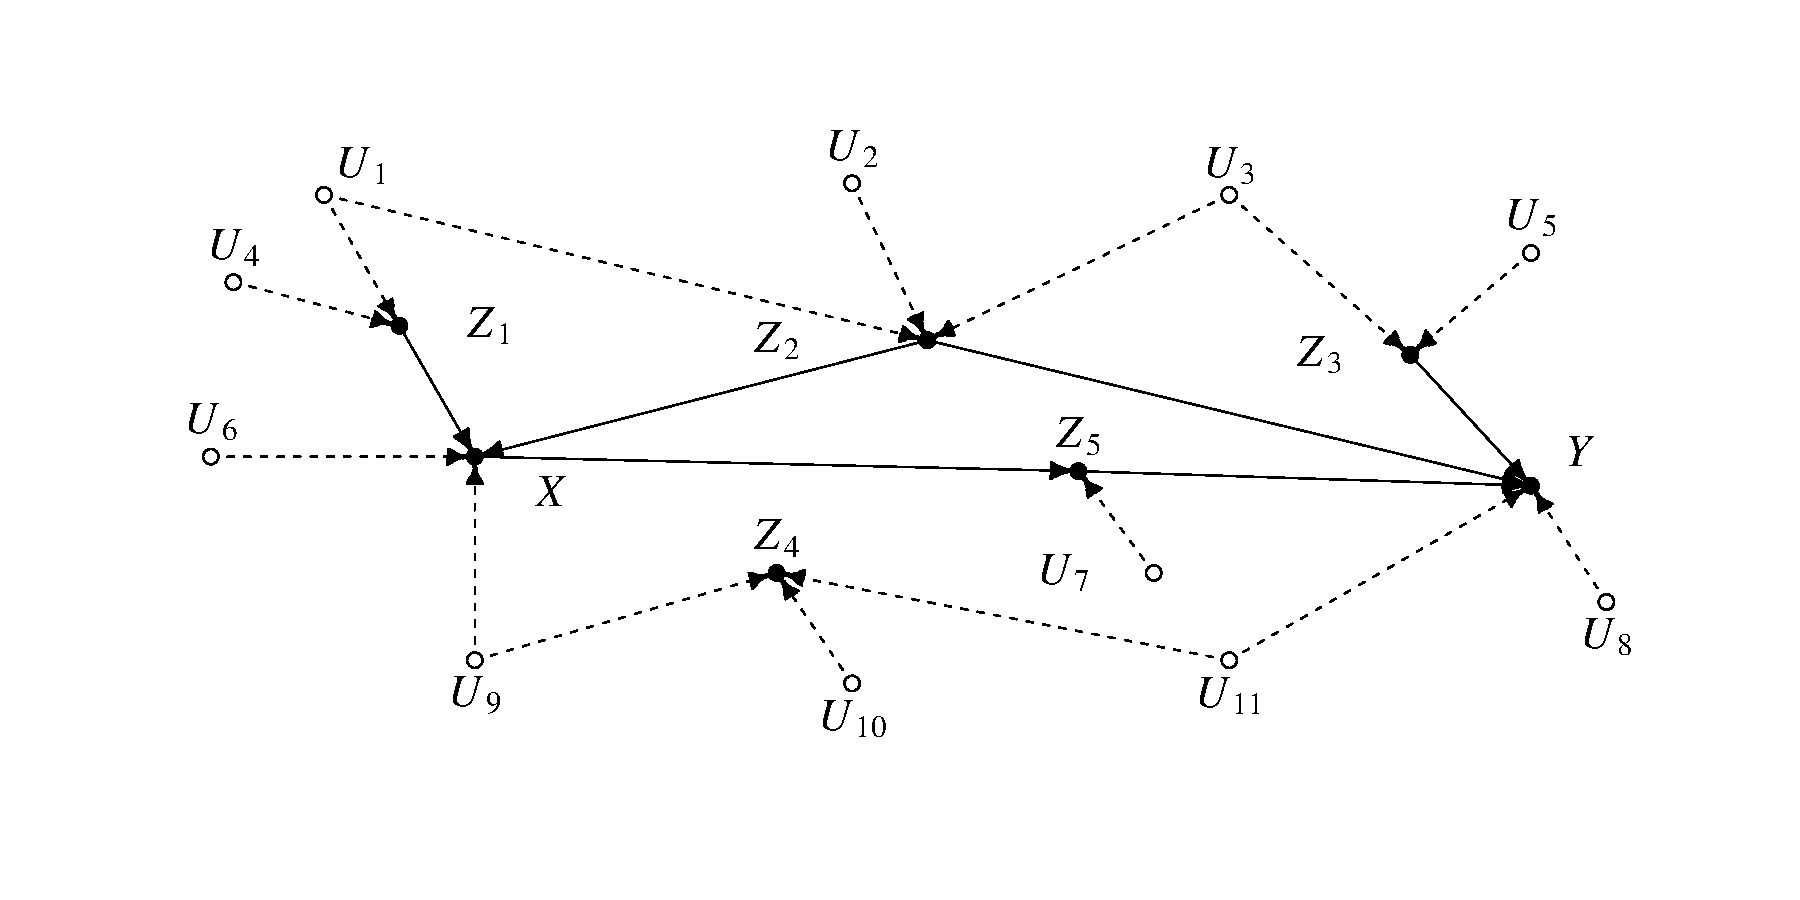
\includegraphics[width=4in,height=3in]{DAG7talk}
%  \end{center}
%  \vspace{-0.275in}
%\end{figure}  
%
%}
%
%
%%\frame{
%%\frametitle{Graphs and Potential Outcomes}
%
%%\begin{figure}[ht]
%%  \begin{center}
% %   \includegraphics[width=4in,height=3in]{DAG7subtalk}
%%  \end{center}
%%  \vspace{-0.275in}
%%\end{figure}  
%
%%}
%
%%\frame{
%
%%\begin{definition}[Effect of Action]
%%Let $M$ be a causal model, $\X$ a set of variables in $\V$, and $x$ a
%%particular realization of $\X$. The \emph{effect of action} $do(\X=x)$
%%on $M$ is given by the submodel $M_x$. 
%%\end{definition}
%
%%\begin{definition}[Potential Outcome]
%%Let $\X$ and $\Y$ be two subsets of variables in $ \V$. The
%%\emph{potential outcome} of $\Y$ to action $do(\X=x)$, denoted
%%$\Y_x(u)$ is the solution for $\Y$ of the set of equations $F_x$. 
%%\end{definition}
%
%%}
%
%%\frame{
%%\frametitle{Actions and Potential Outcomes}
%
%%\begin{figure}[ht]
% % \begin{center}
%  %  \includegraphics[width=4in,height=3in]{DAG7subtalk}
% % \end{center}
%  %\vspace{-0.275in}
%%\end{figure}  
%
%%}
%
%
%
%
%\frame{
%\frametitle{Choosing Conditioning Variables}
%
%\begin{definition}[Back-Door Criterion (Pearl (2000, p. 79))]
%\begin{enumerate}
%  \item none of the conditioning variables is post-$X$; and
%  \item $X$ is ``$d$-separated'' from $Y$ by the conditioning variables in the graph formed by
%  deleting all arrows out of $X$. 
%\end{enumerate}
%\end{definition}
%
%\begin{figure}[ht]
%  \begin{center}
%    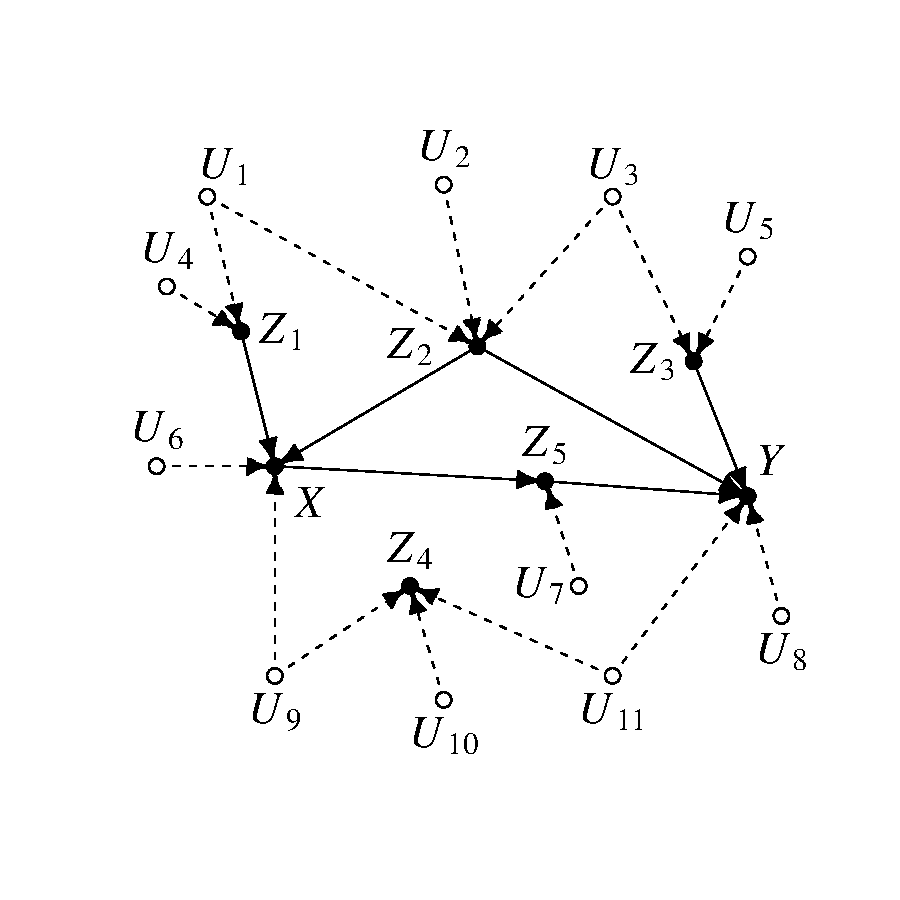
\includegraphics[width=4in,height=2in]{DAG7-full-0.pdf}
%  \end{center}
%  \vspace{-0.275in}
%\end{figure}  
%}
%
%\frame{
%\frametitle{BD1: Don't condition on post-treatment variables}
%
%\begin{figure}[ht]
%  \begin{center}
%    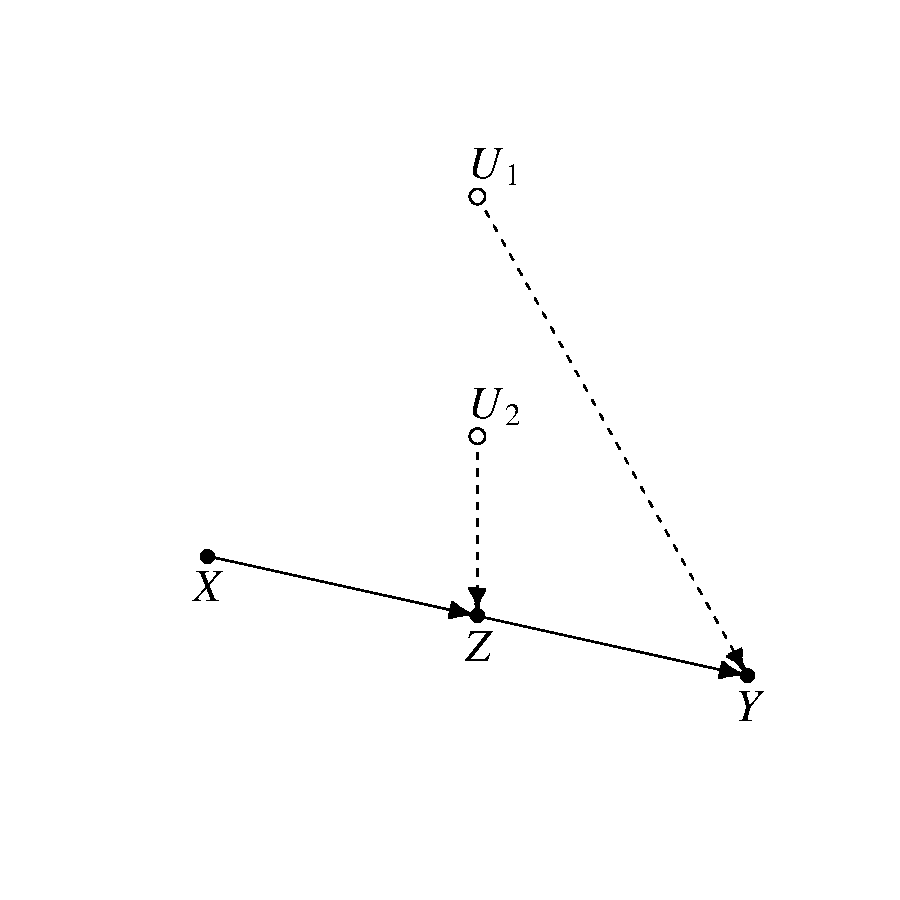
\includegraphics[width=4in,height=2in]{DAGpost0.pdf}
%  \end{center}
%  \vspace{-0.275in}
%\end{figure}  
%
%
%}
%
%\frame{
%\frametitle{BD1: Don't condition on descendants of $X$}
%
%\begin{figure}[ht]
%  \begin{center}
%    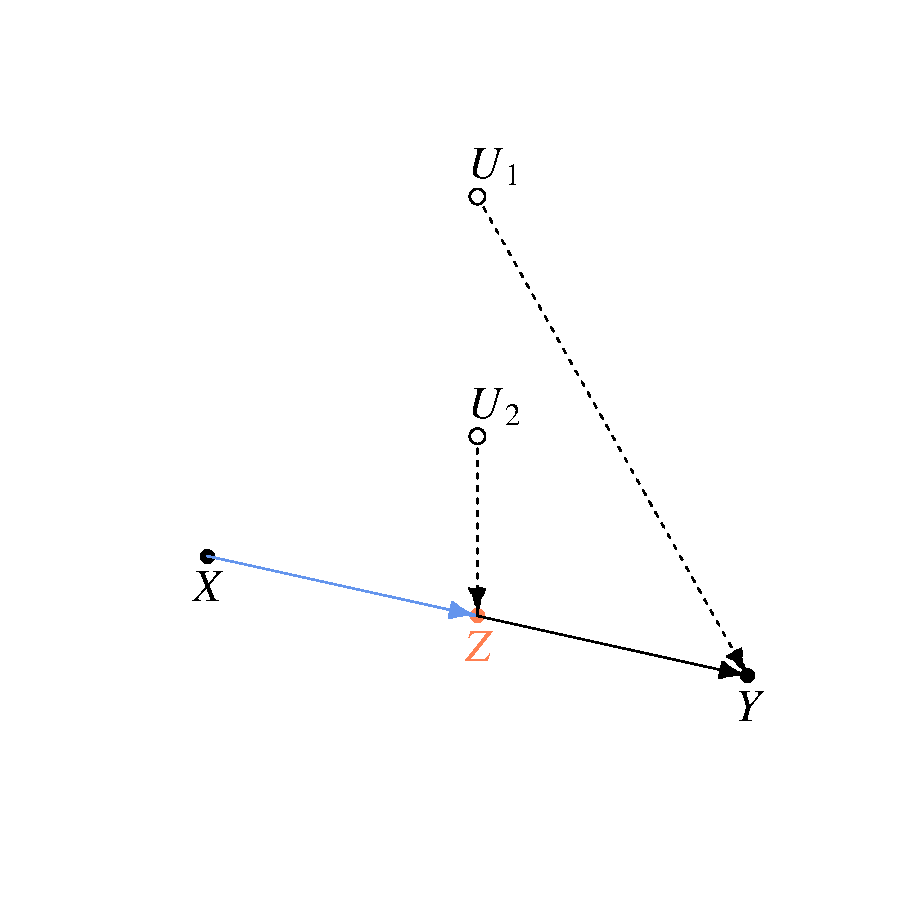
\includegraphics[width=4in,height=2in]{DAGpost1.pdf}
%  \end{center}
%  \vspace{-0.275in}
%\end{figure}  
%
%
%}
%
%\frame{
%\frametitle{BD1: Don't condition on descendants of $X$}
%
%\begin{figure}[ht]
%  \begin{center}
%    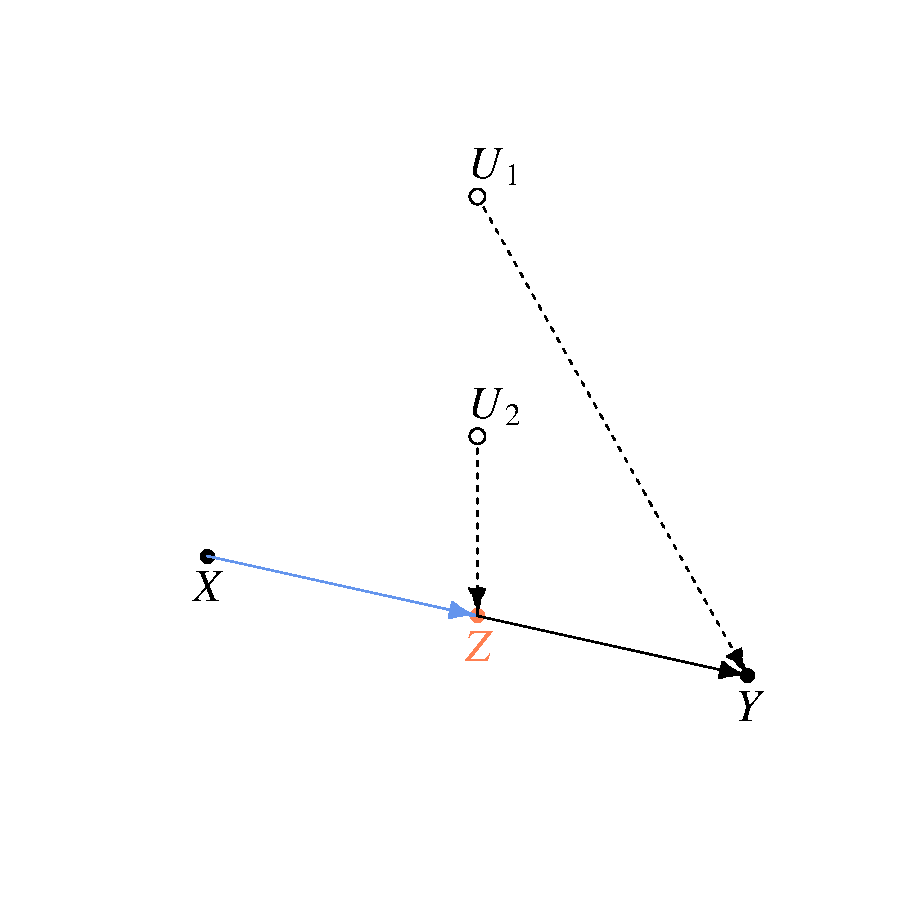
\includegraphics[width=2in,height=1in]{DAGpost1.pdf}
%  \end{center}
%  \vspace{-0.275in}
%\end{figure}  
%
%\begin{quote}
%In sum, if the variable we leave out is positively correlated with the variable we include and also has itself a positive effect on the dependent variable, then our mispecified model will produce an upward-biased estimator of the effect of $X_1$ on $Y$. [Ashenfelter, Levine, and Zimmerman, p. 2003]%\cite[p. 449]{Kme86}
%\end{quote}
%
%}
%
%
%
%\frame{
%\frametitle{BD2: $X$ is $d$-separated from $Y$ by the conditioning variables in the graph formed by
%  deleting all arrows out of $X$.}
%
%%\begin{align*}
%%P(x,y,\z,\u) &= \left( \prod_{j=1}^{11} P(u_j)\right) \cdot P(z_1|u_1,u_4) \cdot P(z_2|u_1,u_2,u_3) \\
%%&\quad\quad \cdot P(z_3|u_3,u_5) \cdot P(z_4|u_9,u_{10},u_{11}) \cdot P(x|z_1,z_2,u_6,u_9) \\
%%&\quad\quad \cdot P(z_5|x,u_1,u_2,u_3) \cdot P(y|z_2,z_3,z_5,u_8,u_{11}) 
%%\end{align*}
%
%\begin{definition}[$d$-Separation (Pearl (2000, p. 16))]
%
%\begin{enumerate}
%  \item $X$ is $d$-Separated from $Y$ if all paths are blocked
%  \item paths are blocked by ``unconditioned colliders'' or conditioned non-colliders
%\end{enumerate}
%\end{definition}
%
%\vspace{.5cm}
%
%$d$-Separation allows conditional independence relations to be read from a DAG consistent with a probabilistic model.
%
%}
%
%\frame{
%\frametitle{Example: Sufficient Conditioning Sets}
%
%\begin{figure}[ht]
%  \begin{center}
%    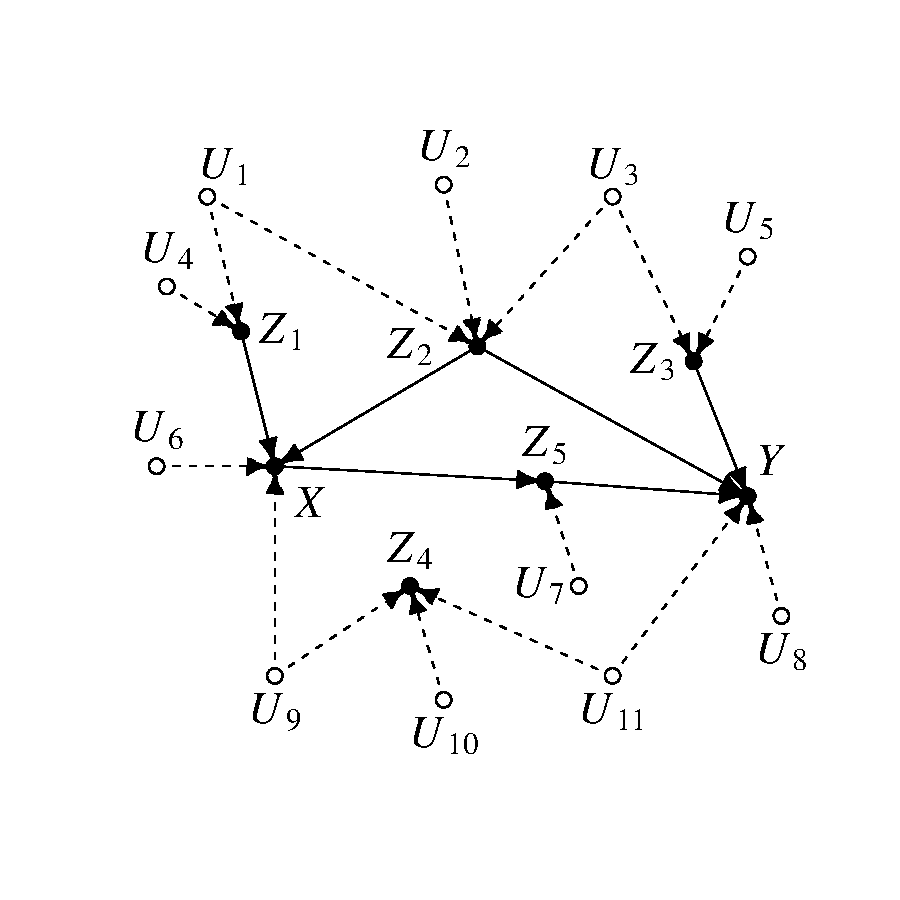
\includegraphics[width=4in,height=2in]{DAG7-full-0.pdf}
%  \end{center}
%  \vspace{-0.275in}
%\end{figure}  
%
%Remove arrows out of $X$. 
%
%}
%
%\frame{
%\frametitle{Example: Sufficient Conditioning Sets}
%
%\begin{figure}[ht]
%  \begin{center}
%    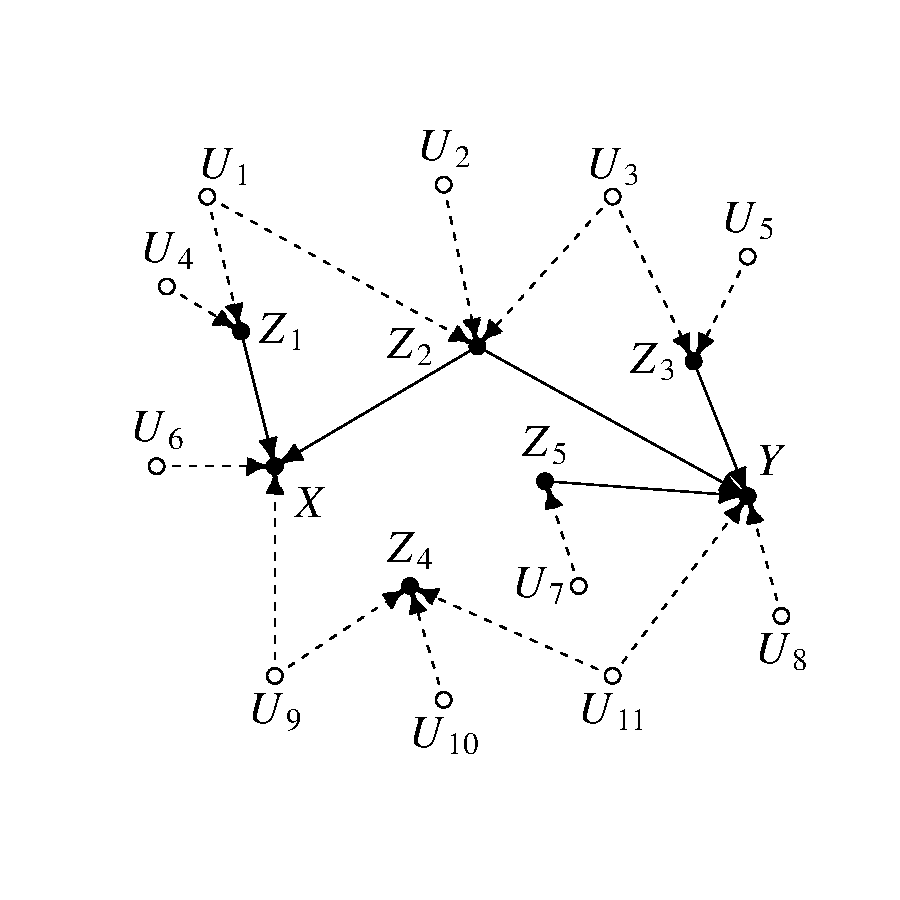
\includegraphics[width=4in,height=2in]{DAG7-nofront-0.pdf}
%  \end{center}
%  \vspace{-0.275in}
%\end{figure}  
%
%Recall that paths are blocked by  ``unconditioned colliders'' or conditioned non-colliders
%
%}
%
%\frame{
%\frametitle{Example: Sufficient Conditioning Sets}
%
%\begin{figure}[ht]
%  \begin{center}
%    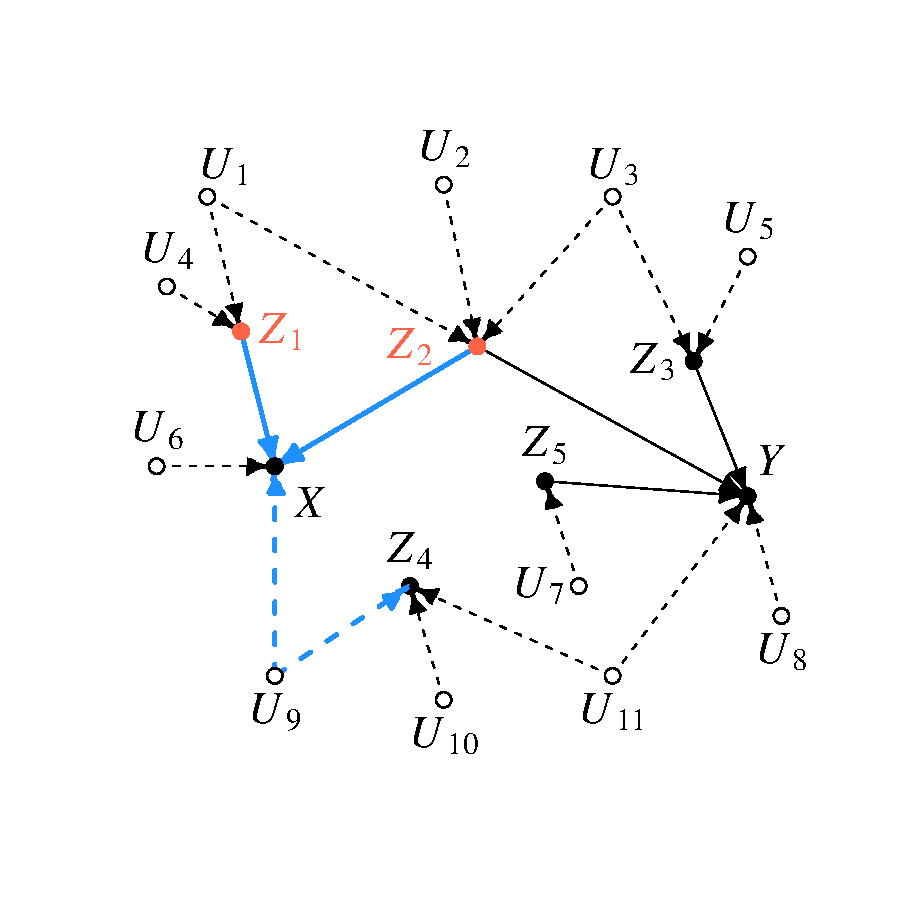
\includegraphics[width=4in,height=2in]{DAG7-nofront-1.pdf}
%  \end{center}
%  \vspace{-0.275in}
%\end{figure}  
%
%Recall that paths are blocked by  ``unconditioned colliders'' or conditioned non-colliders
%
%}
%
%\frame{
%\frametitle{Example: Sufficient Conditioning Sets}
%
%\begin{figure}[ht]
%  \begin{center}
%    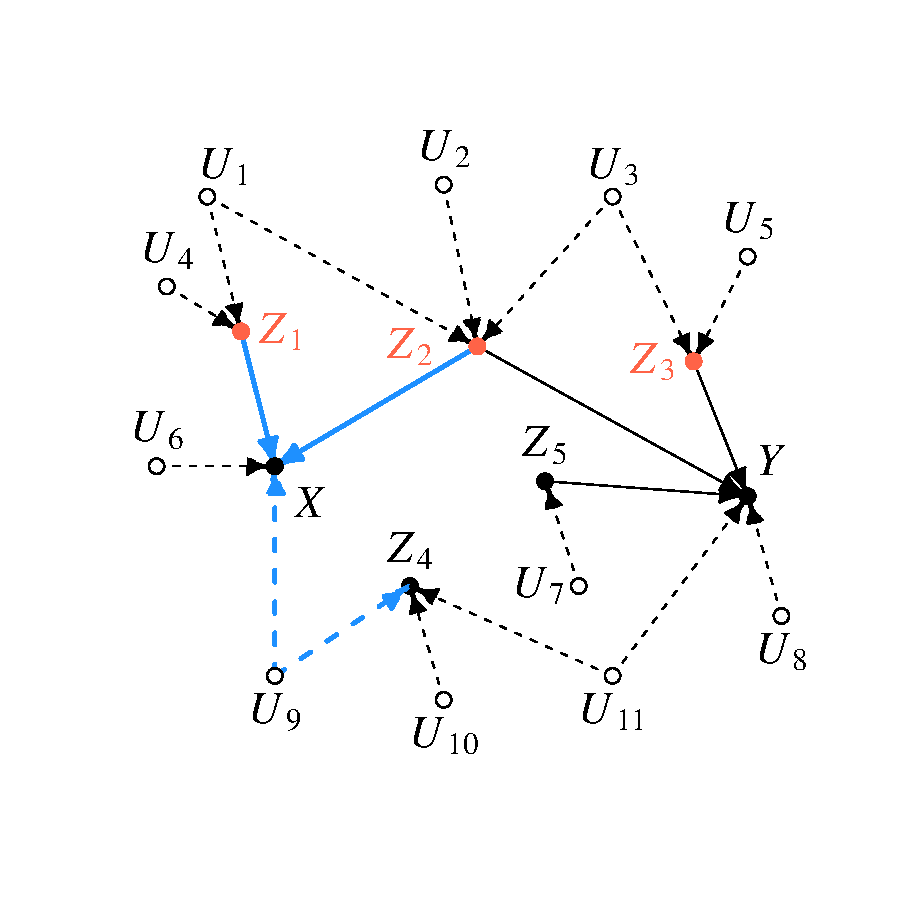
\includegraphics[width=4in,height=2in]{DAG7-nofront-2.pdf}
%  \end{center}
%  \vspace{-0.275in}
%\end{figure}  
%
%Recall that paths are blocked by  ``unconditioned colliders''  or conditioned non-colliders
%
%}
%
%\frame{
%\frametitle{Example: Sufficient Conditioning Sets}
%
%\begin{figure}[ht]
%  \begin{center}
%    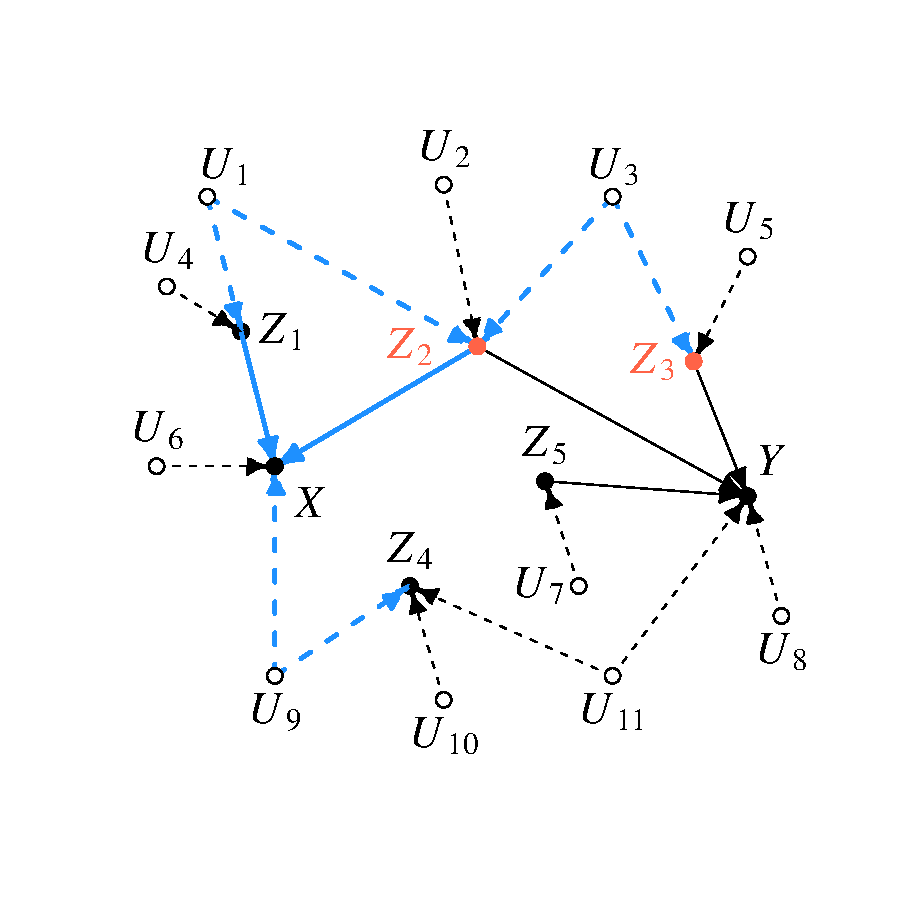
\includegraphics[width=4in,height=2in]{DAG7-nofront-3.pdf}
%  \end{center}
%  \vspace{-0.275in}
%\end{figure}  
%
%Recall that paths are blocked by  ``unconditioned colliders'' or conditioned non-colliders
%
%}
%
%\frame{
%\frametitle{Example: Non-sufficient Conditioning Sets}
%
%\begin{figure}[ht]
%  \begin{center}
%    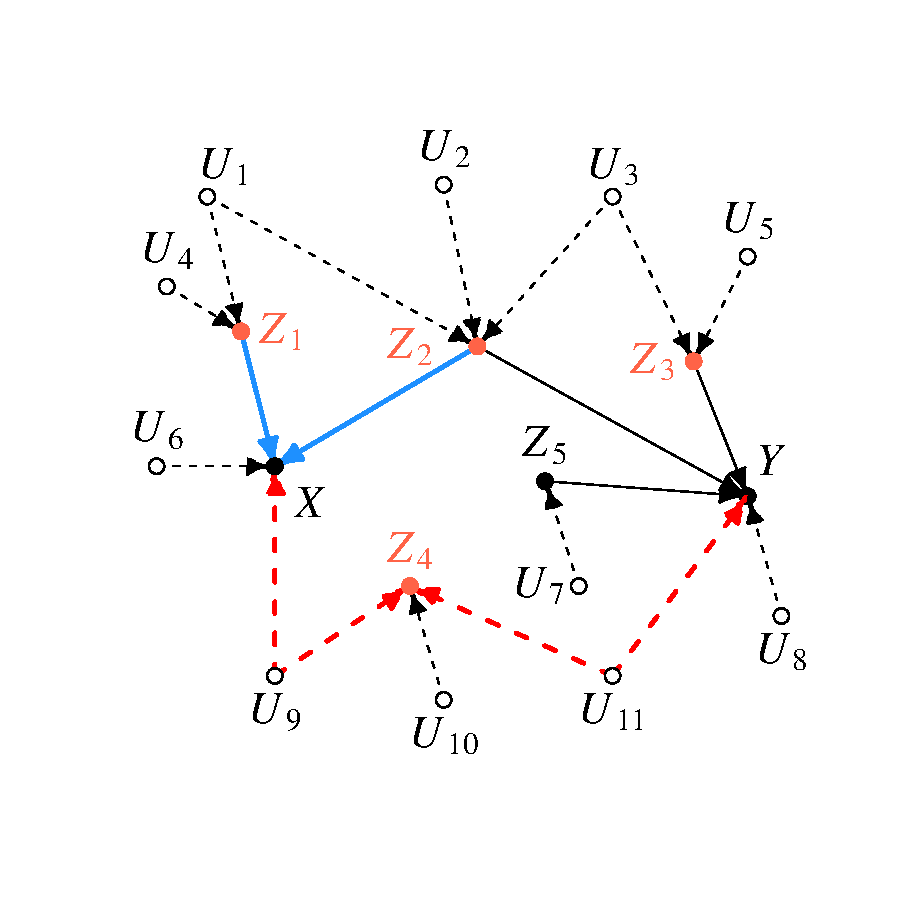
\includegraphics[width=4in,height=2in]{DAG7-nofront-4.pdf}
%  \end{center}
%  \vspace{-0.275in}
%\end{figure}  
%
%Recall that paths are blocked by  ``unconditioned colliders'' or conditioned non-colliders
%
%}
%
%\frame{
%\frametitle{Example: Non-sufficient Conditioning Sets}
%
%\begin{figure}[ht]
%  \begin{center}
%    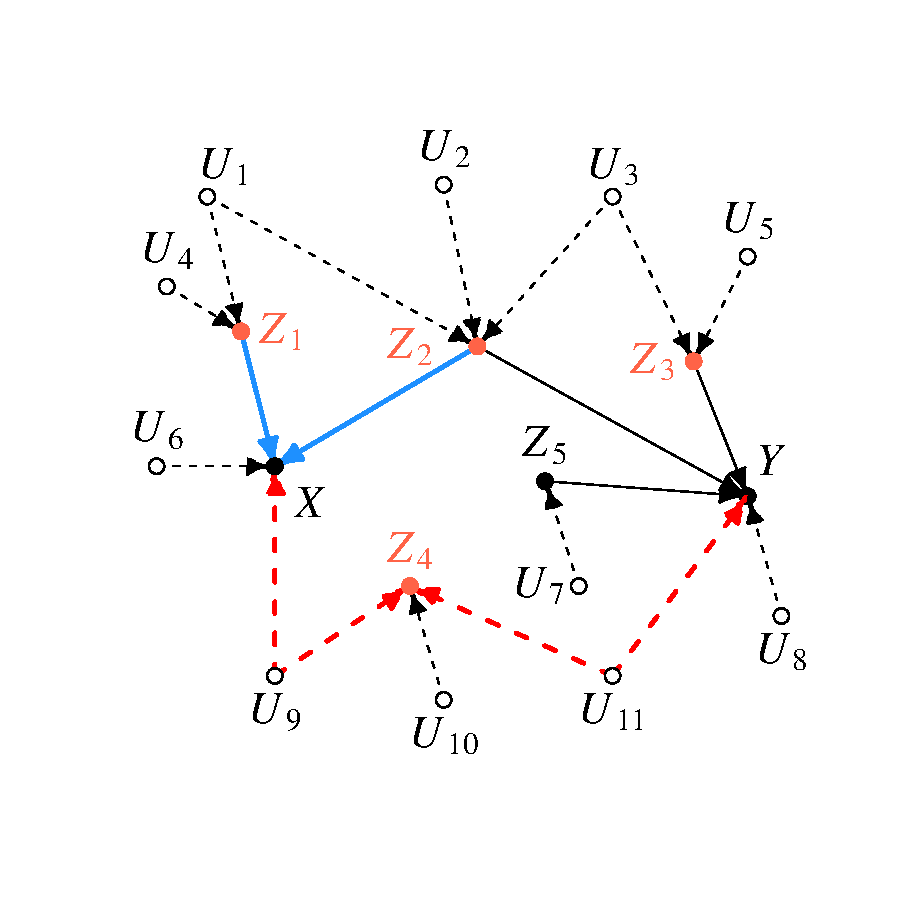
\includegraphics[width=2in,height=1in]{DAG7-nofront-4.pdf}
%  \end{center}
%  \vspace{-0.275in}
%\end{figure}  
%
%\begin{quote}
%The short answer to the questions posed above is that the OLS estimates based on the equation containing too many explanatory variables will indeed be unbiased estimates of the true parameters. [Ashenfelter, Levine, and Zimmerman, p. 187]%\cite[p. 449]{Kme86}
%\end{quote}
%
%%\begin{quote}
%%The conclusion, then, is that if the specification error consists of
%%including some irrelevant explanatory variables in the regression
%%equation, the least squares estimators of the regression coefficients
%%are unbiased but not efficient.  [Kmetka 1986, p. 449]%\cite[p. 449]{Kme86}
%%\end{quote}
%
%}


%\section{Estimation with Regression}


%\frame{
%\frametitle{One Child Legislators in the 105th Congress}
%
%\begin{figure}[ht]
%  \begin{center}
%    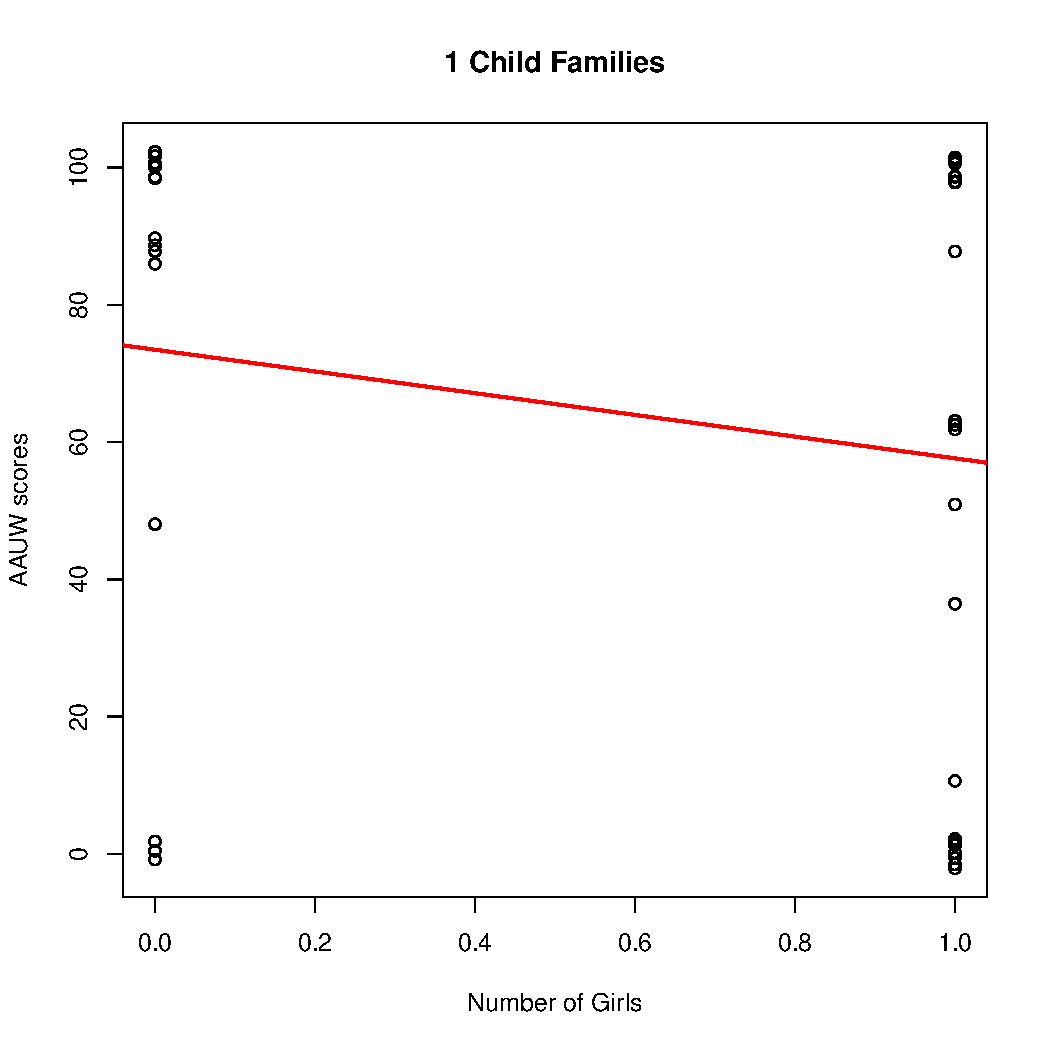
\includegraphics[height=2.5in]{1ch.pdf}
%  \end{center}
%  \vspace{-0.275in}
%\end{figure}  
%Among the subset of one-child legislators, we could adopt the standard potential outcomes approach.
%
%
%}
%
%
%
%\frame{
%\frametitle{Two Children Legislators in the 105th Congress}
%
%\begin{figure}[ht]
%  \begin{center}
%    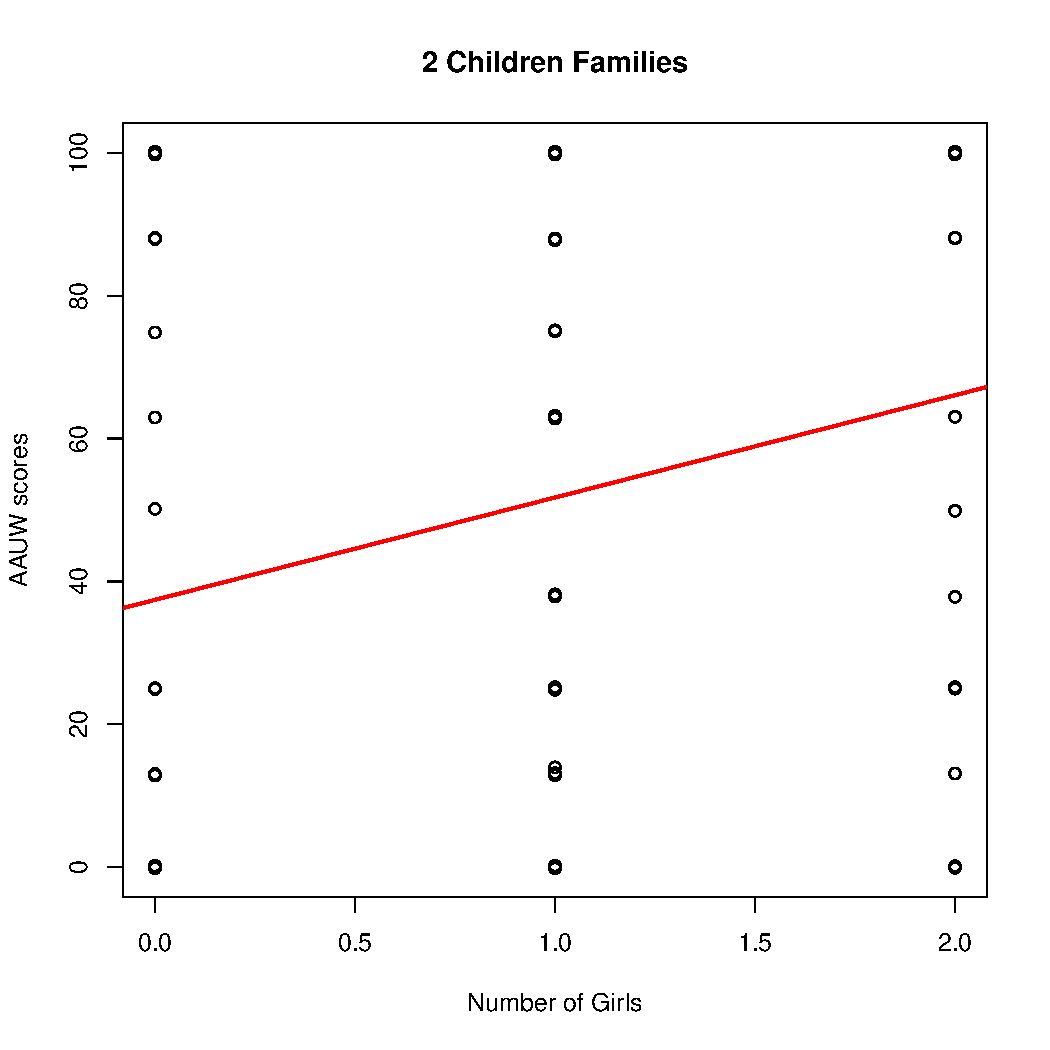
\includegraphics[height=2.5in]{2ch.pdf}
%  \end{center}
%  \vspace{-0.275in}
%\end{figure}  
%How would you construct the potential outcomes table for families with 2 children? \pause
%What assumption is now implicit in the regression?
%
%}
%
%
%\frame{
%Among the subset of 2 children legislators, assume a linear CEF 
%\begin{align*}
%E[Y|T=t] = \beta_0 + \beta_1 \cdot t 
%\end{align*}
%\pause
%When is $\beta_1$ interpretable as the ATE of a one unit increase? 
%\begin{align*}
%\beta_1 &= E[Y|T=t+1]-E[Y|T=t] \text{ for all } t  \\
%&=\onslide<3->{E[Y(t+1)|T=t+1]-E[Y(t)|T=t] \text{ for all } t }\\
%&=\onslide<4->{E[Y(t+1)-Y(t)]  \text{ for all } t }
%\end{align*}
%
%\onslide<5->{This linear approach would also be straightforward for 3 children, 4 children, etc.}\\ 
%
%\vspace{.5cm}
%
%\onslide<6>{What are some ways we could combine these analyses across all legislators?}
%
%}
%
%
%
%\frame{
%Assume a linear additive CEF
%\begin{align*}
%E[Y|T=t,X=x] = \beta_0 + \beta_1 \cdot t + \beta_2 \cdot x
%\end{align*}
%\pause
%
%\vspace{.5cm}
%
%When is $\beta_1$ interpretable as the ATE of a one unit increase? 
%{\footnotesize
%\begin{align*}
%\beta_1 &= \onslide<3->{E[Y|T=t+1,X=x]-E[Y|T=t,X=x] \text{ for all } t,x} \\
%&= \onslide<4->{E_X\left\{E[Y|T=t+1,X=x]-E[Y|T=t,X=x]\right\} \text{ for all } t} \\
%&= \onslide<5->{E_X\left\{E[Y(t+1)|T=t+1,X=x]-E[Y(t)|T=t,X=x]\right\} \text{ for all } t} \\
%&= \onslide<6->{E_X\left\{E[Y(t+1)|X=x]-E[Y(t)|X=x]\right\} \text{ for all } t} \\
%&= \onslide<7->{E_X\left\{E[Y(t+1)-Y(t)|X=x]\right\} \text{ for all } t} \\
%&= \onslide<8->{E[Y(t+1)-Y(t)]  \text{ for all } t} 
%\end{align*}}
%
%}
%
%\frame{
%\frametitle{The Additive Linear Model}
%
%\begin{figure}[ht]
%  \begin{center}
%    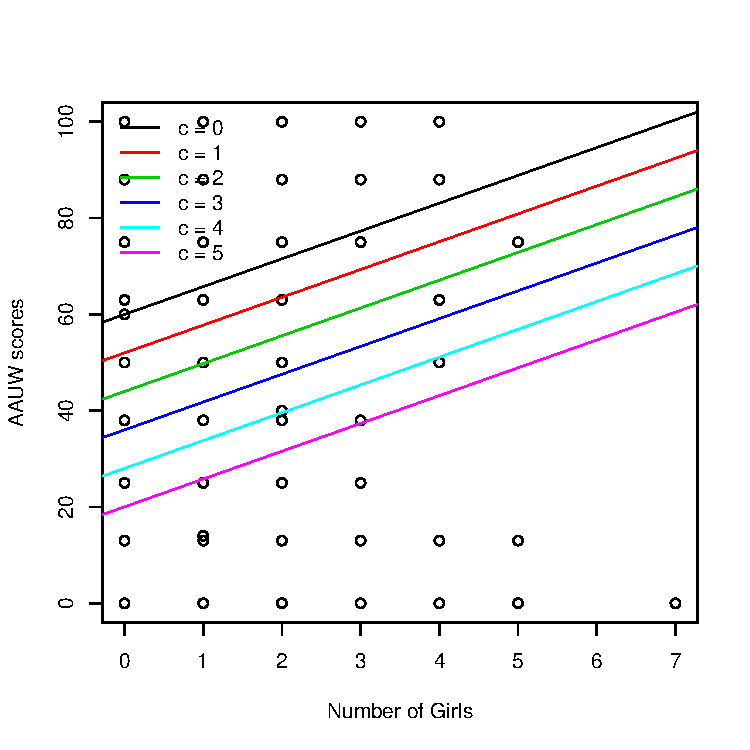
\includegraphics[height=2.5in]{3e.pdf}
%  \end{center}
%  \vspace{-0.275in}
%\end{figure}  
%
%}
%
%\frame{
%\frametitle{The Interactive Linear Model}
%
%
%\begin{align*}
%E[Y|T=t,X=x] &= \onslide<1->{\beta_0 + \beta_1 \cdot t + \beta_2 \cdot x+ \beta_3 \cdot t \cdot x} \\
%&= \onslide<2->{\beta_0 + \bs{(\beta_1 + \beta_3 \cdot x)} \cdot t + \beta_2 \cdot x}
%\end{align*}
%\onslide<2->{When is $(\beta_1 + \beta_3 \cdot x)$ interpretable as the ATE of a one unit increase, conditional on $X=x$?} 
%{\footnotesize
%\begin{align*}
%\onslide<2->{(\beta_1 + \beta_3 \cdot x)} &\onslide<2->{=} \onslide<3->{E[Y|T=t+1,X=x]-E[Y|T=t,X=x] \text{ for all } t,x}\\
%&\onslide<2->{=} \onslide<4->{E[Y|T=t+1,X=x]-E[Y|T=t,X=x] \text{ for all } t } \\
%&\onslide<2->{=} \onslide<5->{E[Y(t+1)|T=t+1,X=x]-E[Y(t)|T=t,X=x] \text{ for all } t} \\
%&\onslide<2->{=} \onslide<6->{E[Y(t+1)|X=x]-E[Y(t)|X=x] \text{ for all } t}  \\
%&\onslide<2->{=} \onslide<7->{E[Y(t+1)-Y(t)|X=x]\ \text{ for all } t} 
%\end{align*}}
%
%}
%
%
%
%\frame{
%\frametitle{The Interactive Linear Model}
%
%\begin{figure}[ht]
%  \begin{center}
%    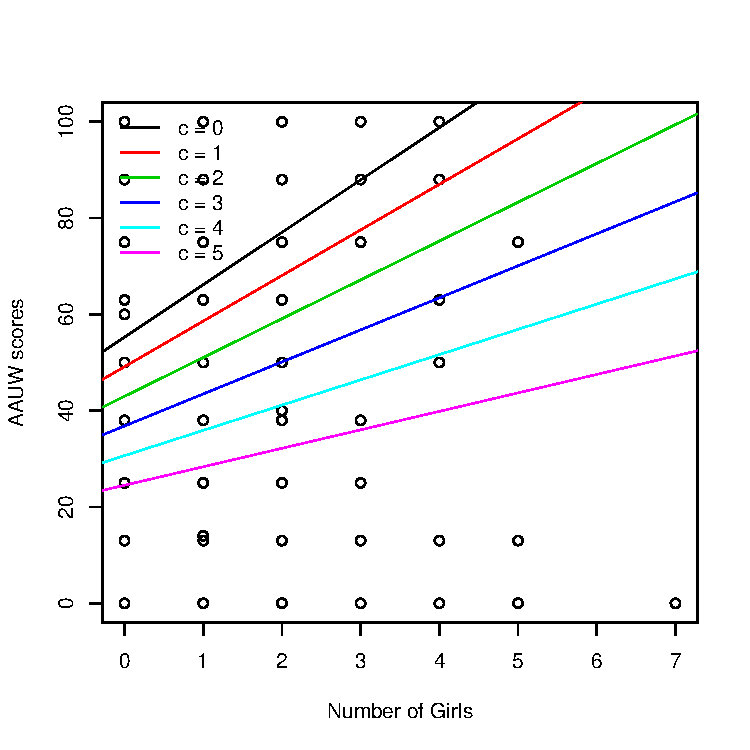
\includegraphics[height=2.5in]{3f.pdf}
%  \end{center}
%  \vspace{-0.275in}
%\end{figure}  
%
% \pause
%
%What would the picture look like if we used a more general model (for which the interactive model and Equation 1 of Washington (2008) are special cases)?
%
%
%
%}
%
%
%\frame{
%\frametitle{Standardization in the Interactive Linear Model}
%
%When is $\beta_1 + \beta_3 \cdot E_X\left\{X \right\}$ interpretable as the ATE of a one unit increase? 
%\begin{align*}
%\beta_1 &+ \beta_3 \cdot E_X\left\{X \right\} = \onslide<2->{E_X\left\{\beta_1 + \beta_3 \cdot X \right\}} \\
%&= \onslide<3->{E_X\left\{E[Y|T=t+1,X=x]-E[Y|T=t,X=x]\right\}}\\
%&= \onslide<4->{E_X\left\{E[Y(t+1)|T=t+1,X=x]-E[Y(t)|T=t,X=x]\right\}} \\
%&= \onslide<5->{E_X\left\{E[Y(t+1)|X=x]-E[Y(t)|X=x]\right\}}\\
%&= \onslide<6->{E_X\left\{E[Y(t+1)-Y(t)|X=x]\right\}} \\
%&= \onslide<7->{E[Y(t+1)-Y(t)]} 
%\end{align*}
%
%}
%
%\frame{
%\frametitle{Standardization in the Interactive Linear Model}
%
%\begin{figure}[ht]
%  \begin{center}
%    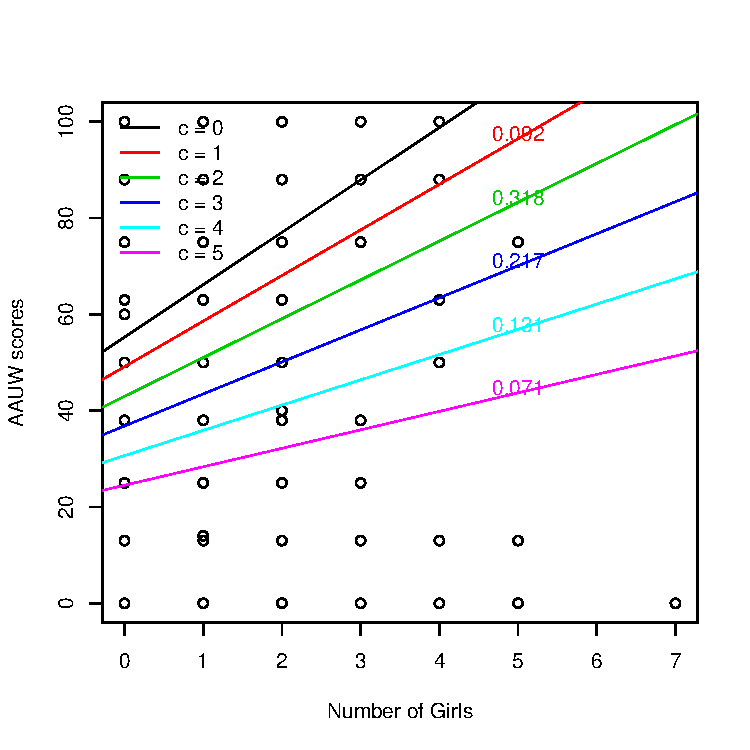
\includegraphics[height=2.5in]{3ff.pdf}
%  \end{center}
%  \vspace{-0.275in}
%\end{figure}  
%
%
%}
%
%\section{Additive vs Interactive}
%
%
%\frame{
%\frametitle{Simple Regression}
%
%Don't use simple regression with a conditionally randomized experiment or a conditionally randomized natural experiment! 
%
%\vspace{.5cm}
%
%
%Leads to omitted variable bais.
%
%}
%
%\frame{
%\frametitle{Additive vs Interactive (Binary $T$ and Binary $X$)}
%
%\begin{align*}
%E[Y|T=t,X=x] &= \beta_0 + \beta_1 \cdot t + \beta_2 \cdot x \\
%E[Y|T=t,X=x] &= \beta_0 + \beta_1 \cdot t + \beta_2 \cdot x + + \beta_3 \cdot t \cdot x
%\end{align*}
%
%\begin{itemize}
%\item Interactive requires standardization ($P(X=1)CATE_{X=1} + P(X=0)CATE_{X=0}$) but provides an estimate of ATE.
%\item Additive is easier (just report $\beta_1$), but it provides an estimate of a weighted ATE.
%\end{itemize}
%
%}
%
%\begin{frame}[fragile]
%
%\begin{verbatim}
%cong12 <- subset(cong, totchi==1 | totchi==2)
%cong12$anygirls <- cong12$ngirls > 0
%cong12$twochi <- cong12$totchi==2
%
%> lm(aauw ~ anygirls * I(twochi - mean(twochi)), data=cong12)
%(Intercept)   anygirlsTRUE    I(twochi - mean(twochi))  
%     47.742         7.893                         -33.181  
%anygirlsTRUE:I(twochi - mean(twochi))  
%                               30.595  
%
%> lm(aauw ~ anygirls + twochi, data=cong12)
% (Intercept)  anygirlsTRUE    twochiTRUE  
%      60.001         5.719       -12.501  
%
%\end{verbatim}
%\end{frame}
%
%\begin{frame}[fragile]
%\frametitle{ATE}
%\begin{verbatim}
%> lm(aauw ~ anygirls * I(twochi - mean(twochi)), data=cong12)
%(Intercept)   anygirlsTRUE    I(twochi - mean(twochi))  
%     47.742         7.893                         -33.181  
%anygirlsTRUE:I(twochi - mean(twochi))  
%                               30.595
%                               
%mod <- lm(aauw ~ anygirls * twochi ,data=cong12)
%
%p0 <- (1-mean(cong12$twochi))
%p1 <- mean(cong12$twochi)
%
%mod$coef[2]*p0 + 
%sum(mod$coef[c(2,4)])*p1
%    7.893438 
%\end{verbatim}
%\end{frame}
%
%\begin{frame}[fragile]
%\frametitle{Weighted ATE}
%\begin{verbatim}
%> lm(aauw ~ anygirls + twochi, data=cong12)
% (Intercept)  anygirlsTRUE    twochiTRUE  
%      60.001         5.719       -12.501  
%
%mod <- lm(aauw ~ anygirls * twochi ,data=cong12)
%    
%w0 <- p0*mean(cong12$anygirls[cong12$twochi==0])*
%(1-mean(cong12$anygirls[cong12$twochi==0]))
%w1 <- p1*mean(cong12$anygirls[cong12$twochi==1])*
%(1-mean(cong12$anygirls[cong12$twochi==1]))
%
%mod$coef[2]*(w0/(w0+w1)) + 
%sum(mod$coef[c(2,4)])*(w1/(w0+w1))
%     5.71872 
%\end{verbatim}
%\end{frame}
%
%
%\frame{
%\frametitle{Additive vs Interactive (Binary $T$ and general $X_1,X_2, ...$)}
%
%
%With binary $T$ and general $X_1, X_2, ...$ 
%\begin{align*}
%E[Y|T=t,X=x] &= \beta_0 + \beta_1 \cdot t + \beta_2 \cdot x_1 + \beta_3 \cdot x_2 + ...  \\
%E[Y|T=1,X=x] &= f_1(x_1,x_2,...) \\
%E[Y|T=0,X=x] &= f_0(x_1,x_2,...) \\
%E_{X}[f_1(x_1,x_2,...)) &- f_0(x_1,x_2,...)]
%\end{align*}
%
%\begin{itemize}
%\item Interactive requires standardization (fit a model to the treated units, fit a model to the control units, calculate differences between them for all observations).
%\item Additive is easier (just report $\beta_1$), but it provides an estimate of a weighted ATE.
%\end{itemize}
%
%}
%
%\frame{
%\frametitle{Additive vs Interactive (Non-Binary $T$ and general $X_1,X_2, ...$)}
%
%
%With non-binary $T$ and general $X_1, X_2, ...$ 
%\begin{align*}
%E[Y|T=t,X=x] &= \beta_0 + \beta_1 \cdot t + \beta_2 \cdot x_1 + \beta_3 \cdot x_2 + ...  
%\end{align*}
%
%\begin{itemize}
%\item Interactive requires ... too hard. Come see me if you really want to try.
%\item Additive is easier (just report $\beta_1$), but it provides an estimate of a weighted-weighted ATE.
%\end{itemize}
%
%}
%


%\frame{
%\frametitle{Summary}
%
%\begin{itemize}
%\item The classical advice about choosing conditioning variables can lead to post-treatment bias or M-bias. \pause
%\item Condition on ``confounding'' variables (as defined by the backdoor criterion). \pause
%\item Regression can be used for causal inference, however \pause
%\begin{itemize}
%\item be aware of the consequences of linearity assumptions \pause
%\item be aware of the consequences of additivity assumptions 
%\end{itemize}
%\end{itemize}
%
%}

%\frame{
%\frametitle{Next Week}
%
%Observational Studies with Measured Confounding
%
%\begin{itemize}
%\item Assessing Overlap and Balance 
%\item Revising the Question of Interest 
%\item Relaxing Linearity and Additivity
%\item Bounding and Sensitivity Analysis for Unmeasured Confounding
%\end{itemize}
%
%\vspace{.5cm}
%
%Things to do:
%\begin{itemize}
%\item problem set 
%\item the reading and the reading quiz (see updated syllabus)
%\item annotations
%\end{itemize}
%
%
%}
%
%
\end{document}




%%%%%%%%%%%%%%%%%%%%%%%%%%%%%%

